\documentclass[a4paper,fleqn]{cas-sc}

\usepackage[numbers]{natbib}
\usepackage{algorithm}
\usepackage{algorithmic}
\usepackage{amsmath}
\usepackage{amssymb}
\usepackage{graphicx}

% Bypass missing thumbnails for cas-sc
\makeatletter
\def\@corref#1{\textsuperscript{\@fnsymbol{#1}}\@corref@}
\makeatother
\usepackage{float}
\usepackage{booktabs}
\usepackage{multirow}
\usepackage{tabularx}
\usepackage{lineno}
\usepackage{placeins}



\newtheorem{theorem}{Theorem}
\newtheorem{lemma}{Lemma}

\begin{document}
\let\WriteBookmarks\relax
\def\floatpagepagefraction{1}
\def\textpagefraction{.001}

\shorttitle{High-Order Spectral Method for Time-Fractional Equations}
\shortauthors{A.S. Berdyshev et~al.}

\title [mode = title]{A High-Order Chebyshev Spectral Method for the Time-Fractional Wave Equation with Memory: Rigorous Stability Analysis and Fast Evaluation}

\author[1,2]{A.S. Berdyshev}

\author[1,2]{Zh.A. Abdiramanov}
\cormark[1]
\ead{a.janars@gmail.com}

\author[1]{N. Adil}

\address[1]{Department of Mathematics and Mathematical Modelling, Faculty of Mathematics, Physics and Informatics, Abai Kazakh National Pedagogical University, Almaty 050010, Kazakhstan}
\address[2]{Institute of Information and Computational Technologies, Science Committee of the Ministry of Science and Higher Education, Almaty 050010, Kazakhstan}

\cortext[cor1]{Corresponding author}

\begin{abstract}
The paper is devoted to the efficient and rigorous numerical solution of a one-dimensional hyperbolic wave equation featuring a Caputo fractional time derivative, which models memory effects in viscoelastic media. A fully discrete high-order scheme is developed using the Chebyshev spectral collocation method on the spatial grid of Chebyshev--Gauss--Lobatto (CGL) nodes and the implicit Newmark scheme in time equipped with the $L1$ formulation for the memory kernel. We provide a complete and rigorous proof of the energy stability, establishing an a priori estimate under a Lipschitz condition on the nonlinear source and proving the positive-definiteness of the memory kernel via the Bochner--Herglotz theorem. Using the Lax equivalence principles and the discrete energy method, spatial-temporal convergence estimates are derived, confirming $\mathcal{O}(\Delta t^{2-\alpha})$ temporal accuracy and exponential $\mathcal{O}(N^{-m})$ spatial accuracy for smooth solutions. To overcome the dense history dependence, the computational complexity of the memory integral is reduced from $\mathcal{O}(N_t^2)$ to $\mathcal{O}(N_t N_e)$ via the sum-of-exponentials (SOE) algorithm. Numerical experiments validate the theoretical convergence rates, demonstrate the exponential spatial convergence for smooth profiles, explore the degradation and recovery of accuracy for singular phenomena using graded temporal meshes, and highlight the dramatic efficiency acceleration achieved by the SOE algorithm.
\end{abstract}

\begin{keywords}
wave equation with memory \sep Caputo fractional derivative \sep spectral collocation method \sep Chebyshev--Gauss--Lobatto nodes \sep energy stability \sep convergence analysis \sep fast memory evaluation
\end{keywords}

\maketitle

\section{Introduction}
Time-fractional wave equations model memory effects arising from power-law relaxation and creep in viscoelastic media, anomalous dispersion in fluid-saturated porous rocks, and frequency-dependent attenuation in biological tissues~\cite{ref13,ref14,ref17,ref18}. Replacing integer-order damping with a Caputo fractional derivative yields a convolution integral that captures these hereditary phenomena~\cite{ref19,ref20}. The development of accurate, stable, and efficient numerical methods for such non-local problems remains an active area of research in computational mathematics.

Spectral collocation methods achieve exponential convergence for smooth solutions on canonical domains~\cite{ref5,gottlieb1977}, complementing finite difference~\cite{ref1,ref3,ref9} and finite element~\cite{ref2,mustapha2015} approaches that are preferred for complex geometries. Fractional spectral elements and related high-order approaches have been actively developed~\cite{zayernouri2014, shiyapov2026high}; the well-posedness and regularity theory was established in~\cite{sakamoto2011,mclean2010,bazhlekova2013}. A critical computational bottleneck is the dense convolution history: the standard $L1$ discretisation of the memory integral requires $\mathcal{O}(N_t^2)$ operations, which limits practical applicability and motivates the use of fast algorithms~\cite{ref6,baffet2017}.

Despite these advances, a rigorous coupled stability and convergence analysis of Chebyshev spectral collocation with an $L1$-type Newmark temporal scheme, complemented by the sum-of-exponentials (SOE) fast evaluation, has not been presented in the literature. The \emph{main contributions} of this work are: (i)~formulation of a fully discrete high-order scheme combining Chebyshev spatial discretisation with an implicit Newmark temporal integrator equipped with the $L1$ memory approximation; (ii)~discrete energy stability and spatio-temporal convergence estimates under explicit assumptions on the spatial operator and memory kernel; (iii)~integration of the SOE algorithm~\cite{ref6}, reducing the memory complexity from $\mathcal{O}(N_t^2)$ to $\mathcal{O}(N_t N_e)$; and (iv)~a systematic numerical study of exponential spatial convergence, fractional temporal convergence rates, and the treatment of weakly singular solutions via graded meshes~\cite{stynes2017,liao2018sharp}. All numerical experiments employ the $L1$ approximation of the Caputo memory integral, achieving $\mathcal{O}(\Delta t^{2-\alpha})$ temporal convergence for solutions with sufficient regularity.

The paper is organised as follows. Section~2 formulates the problem and the discrete scheme. Section~3 presents the stability and convergence theorems. Section~4 reports numerical experiments. Section~5 contains conclusions.

\subsection{Model Description}\label{sec:model}

We consider the one-dimensional time-fractional wave equation on $\Omega = (0, L)$, $L > 0$:
\begin{linenomath}
\begin{equation}\label{eq:wave}
\frac{\partial^2 u}{\partial t^2} - c^2 \frac{\partial^2 u}{\partial x^2} + \int_0^t \kappa(t-s) \frac{\partial u}{\partial s}(x, s) \, ds = f(x, t, u), \quad x \in (0,L),\; t \in (0, T),
\end{equation}
\end{linenomath}
where $c > 0$ is the wave speed and $f(x, t, u)$ satisfies the Lipschitz condition $|f(x,t,u_1) - f(x,t,u_2)| \le L_f |u_1 - u_2|$. The memory kernel $\kappa(t) = \frac{\gamma}{\Gamma(1-\alpha)} t^{-\alpha}$, $0 < \alpha < 1$, $\gamma > 0$, corresponds to the Caputo fractional derivative. The equation is supplemented with initial conditions $u(x, 0) = u_0(x)$, $\partial_t u(x, 0) = v_0(x)$ and homogeneous Dirichlet boundary conditions $u(0, t) = u(L, t) = 0$.

\section{Problem Statement}\label{sec:existence}
The inclusion of the memory kernel induces energy dissipation~\cite{ref15}. The total energy is $E(t) = \frac{1}{2} \int_0^L [(\partial_t u)^2 + c^2 (\partial_x u)^2]\, dx$. Well-posedness under sufficient regularity of the data ($u_0 \in H_0^1 \cap C^2$, $v_0 \in L^2 \cap C^1$) and positive definiteness of $\kappa$ follows from standard energy estimates and Gronwall's lemma; see Appendix~\ref{app:existence} and~\cite{sakamoto2011,mclean2010}.

\subsection{CGL Grid and Temporal Discretization}\label{sec:space_disc}
The spatial domain is discretized using $N+1$ Chebyshev--Gauss--Lobatto (CGL) nodes~\cite{ref5}:
\begin{linenomath}
\begin{equation}\label{eq:cgl}
  x_j = \frac{L}{2} \left[1 - \cos\left(\frac{\pi (N-j)}{N}\right)\right], \quad j = 0, 1, \ldots, N,
\end{equation}
\end{linenomath}
with minimal spacing $h_{\min} = \mathcal{O}(N^{-2})$ near the boundaries. The temporal domain is discretized into uniform steps $t_n = n \Delta t$, $\Delta t = T/N_t$. The second time derivative is approximated by the standard $\mathcal{O}(\Delta t^2)$ central difference.

The memory integral is discretized using the $L1$ scheme~\cite{ref21,jin2016}. Setting $a_0 = \Delta t^{-\alpha}/\Gamma(2-\alpha)$, the Caputo fractional derivative at $t_n$ is approximated by:
\begin{linenomath}
\begin{equation}\label{eq:l2sigma}
\int_0^{t_n}\kappa(t_n-s)\,\dot{u}(s)\,ds \approx a_0\,\gamma\sum_{k=0}^{n-1}w_{k}\,(U^{n-k}-U^{n-1-k}),
\end{equation}
\end{linenomath}
where the weights are $w_k = (k+1)^{1-\alpha} - k^{1-\alpha}$ for $k \ge 0$. These weights satisfy $w_k > 0$ and are strictly decreasing. On a uniform grid, the $L1$ scheme achieves $\mathcal{O}(\Delta t^{2-\alpha})$ for the memory term~\cite{jin2016,liao2018sharp}. The overall temporal convergence of the coupled Newmark--$L1$ scheme is therefore $\mathcal{O}(\Delta t^{2-\alpha})$, governed by the memory approximation. For solutions with an initial-layer singularity, graded meshes $t_j = T(j/N_t)^r$ maintain optimal rates~\cite{stynes2017,liao2018sharp}.

\subsection{Fast Memory Evaluation via Sum of Exponentials}\label{sec:soe}

The $L1$ convolution sum requires $\mathcal{O}(N_t^2)$ operations over the full simulation. To reduce this cost, we employ the SOE algorithm of Jiang--Zhang~\cite{ref6}, which approximates the $L1$ weights by $N_e$ exponentials: $c_j \approx \sum_{l=1}^{N_e} \hat{c}_l\, e^{-\mu_l t_j}$. The nodes $\mu_l$ and weights $c_l$ are computed via trapezoidal quadrature of the Bromwich integral on a logarithmic grid~\cite{ref6}. The exponential structure enables a one-step recursion for the history accumulators $Z_l^n$:
\begin{linenomath}
\begin{equation}\label{eq:soe_recursion}
  Z_l^{n} = q_l\,Z_l^{n-1} + \delta U^{n-p-1}, \quad q_l = e^{-\mu_l \Delta t},
\end{equation}
\end{linenomath}
where $\delta U^k = U^{k+1}-U^k$. The full memory sum splits into an exact near-history window of width $p$ and the SOE tail:
\begin{linenomath}
\begin{equation}\label{eq:soe_full}
  H^n = \sum_{j=0}^{p-1} c_j\,\delta U^{n-1-j} + \sum_{l=1}^{N_e} c_l\,Z_l^n,
\end{equation}
\end{linenomath}
reducing the per-step cost from $\mathcal{O}(n)$ to $\mathcal{O}(p + N_e)$ and the total cost from $\mathcal{O}(N_t^2)$ to $\mathcal{O}(N_t(p+N_e))$~\cite{ref11,ref10}.

\subsection{Spatial Discretization}\label{sec:spatial_matrices}
The spatial operator $c^2 \partial_{xx}$ is approximated by the Chebyshev spectral differentiation matrix $D$~\cite{ref5,gottlieb1977}. On the physical interval $[0,L]$, the interior block of the second-derivative matrix defines the discrete operator:
\begin{linenomath}
\begin{equation}\label{eq:spectral_semi}
  A = c^2 \tilde{D}^{(2)} \in \mathbb{R}^{(N-1) \times (N-1)}, \qquad \tilde{D}^{(2)} = \bigl[(2/L)\,D\bigr]^2\big|_{\text{interior}},
\end{equation}
\end{linenomath}
where the boundary rows/columns are eliminated to enforce homogeneous Dirichlet conditions. The resulting dense matrix provides exponential convergence $\mathcal{O}(N^{-m})$ for solutions of Sobolev regularity $H^m$~\cite{ref5}.

\section{Theoretical Analysis}\label{sec:analysis}

On the grid defined in Section~\ref{sec:space_disc}, the fully discrete scheme combines the standard second-order central difference for $u_{tt}$ with the Newmark implicit spatial averaging ($\beta=1/4$) and the $L1$ memory quadrature:
\begin{linenomath}
\begin{equation}\label{eq:full_discrete_scheme}
\begin{split}
  \frac{U^{n+1}\!-\!2U^n\!+\!U^{n-1}}{\Delta t^2} - A\bigl[\tfrac{1}{4}U^{n+1}\!+\!\tfrac{1}{2}U^n\!+\!\tfrac{1}{4}U^{n-1}\bigr] + a_0\gamma\,H^{n} = F^{n},
\end{split}
\end{equation}
\end{linenomath}
for $1 \le n \le N_t-1$, where $F^{n} = f(x, t_{n})$ and $a_0 = \Delta t^{-\alpha}/\Gamma(2-\alpha)$. The implicit Newmark averaging $\frac{1}{4}U^{n+1} + \frac{1}{2}U^n + \frac{1}{4}U^{n-1}$ ensures unconditional stability. The $L1$ memory vector $H^n$ is evaluated via the SOE algorithm:
\begin{linenomath}
\begin{equation}\label{eq:discrete_memory_soe}
  H^{n} = \sum_{j=0}^{\min(n-1,\,p-1)} w_j \left(U^{n-j} - U^{n-1-j}\right) + \sum_{l=1}^{N_e} \hat{c}_l\,Z_l^{n},
\end{equation}
\end{linenomath}
where the $L1$ weights $w_k = (k+1)^{1-\alpha}-k^{1-\alpha}$ ($k \ge 0$) are positive and decreasing. The SOE recursion $Z_l^{n} = q_l Z_l^{n-1} + (U^{n-p}-U^{n-1-p})$ remains unchanged.

The two-level scheme~\eqref{eq:full_discrete_scheme} requires $U^0$ and $U^1$. From the initial data $u(x,0)=u_0(x)$ and $\partial_t u(x,0)=v_0(x)$:
\begin{linenomath}
\begin{equation}\label{eq:full_discrete_ic}
  U^0 = u_0,\quad U^1 = U^0 + \Delta t\,v_0 + \tfrac{\Delta t^2}{2}(AU^0 + F^0).
\end{equation}
\end{linenomath}
For $n=1$ the scheme reduces to a two-level step since $U^{-1}$ is known from initialization.
Homogeneous Dirichlet boundary conditions are imposed on the values at the boundary nodes $j=0$ and $j=N$ for any time layer $n \ge 0$:
\begin{linenomath}
\begin{equation}\label{eq:full_discrete_bc}
  U_0^n = 0, \quad U_N^n = 0.
\end{equation}
\end{linenomath}

\subsection{Stability Criteria}

\begin{theorem}[Energy Stability]\label{thm:stability}
Assume the following conditions hold:
\begin{enumerate}
    \item[(i)] The spatial operator $A$ is symmetric negative semi-definite in the Clenshaw--Curtis weighted inner product $\langle U, V \rangle_{CC} = \sum_{j=0}^N w_j^{CC} U_j V_j$, i.e., $\langle -A V, V \rangle_{CC} \ge 0$ for all discrete $V$ satisfying homogeneous Dirichlet boundary conditions.
    \item[(ii)] The $L1$ memory quadratic form is positive semi-definite: $\sum_{n=1}^{m}\langle H^n, \delta\tilde{U}^n\rangle_{CC} \ge 0$ for all $m \ge 1$, where $H^n = \sum_{j=0}^{n-1} w_j\,\delta\tilde{U}^{n-1-j}$ and $\delta\tilde{U}^k = U^{k+1}-U^k$.


    \item[(iii)] The Newmark temporal averaging parameter $\beta = 1/4$.
    \item[(iv)] The source $f(x,t,u)$ is Lipschitz continuous in $u$: there exists $L_f > 0$ such that $\|f(\cdot,t_n,U) - f(\cdot,t_n,V)\|_{CC} \le L_f \|U - V\|_{CC}$ for all discrete $U, V \in V_h$, and the time step satisfies $\Delta t < 1/L_f$.
\end{enumerate}
Then the discrete energy $E^{n+1/2} = \frac{1}{2\Delta t^2}\|U^{n+1}-U^n\|_{CC}^2 + \frac{1}{8}|U^{n+1}+U^n|_A^2$ satisfies, for all $1 \le m \le N_t-1$:
\begin{equation}\label{eq:stability_result}
    E^{m+1/2} \le E^{1/2} \exp(\widetilde{C} \, L_f \, T),
\end{equation}
where $\widetilde{C}$ is a constant depending only on $T$ and $L_f$.
\end{theorem}

\paragraph{Discussion of conditions.} Condition~(i) holds exactly when the Galerkin (variational) form of the spectral method is used. For the collocation formulation, numerical verification confirms that $W^{1/2}AW^{-1/2}$ is symmetric negative semi-definite to machine precision for all $N$ tested ($N \le 64$)~\cite{gottlieb1977}. Condition~(ii) is established for the $L1$ weights in~\cite{ref21,liao2018sharp}.

The proof is given in Appendix~\ref{app:proof_theorem1}.

\subsection{Convergence Properties}

\begin{theorem}[Convergence]\label{thm:convergence}
Under the hypotheses of Theorem~\ref{thm:stability}, assume additionally that the exact solution $u_{\mathrm{exact}} \in C^4(\bar\Omega\times[0,T])$ and the spatial operator $A$ approximates $c^2\partial_{xx}$ with local truncation error $E_{\mathrm{space}}$. Then the global error $e^n = U^n - u_{\mathrm{exact}}^n$ satisfies, for all $1 \le n \le N_t$:
\begin{equation}\label{eq:convergence_result}
    \|e^n\|_{CC} \le C(T)\left( \Delta t^{2-\alpha} + E_{\mathrm{space}} \right),
\end{equation}
where $E_{\mathrm{space}} = \mathcal{O}(N^{-m})$ (yielding exponential decay for analytic solutions) for the Chebyshev spectral method.
\end{theorem}

The detailed proof is given in Appendix~\ref{app:proof_theorem2}.
\section{Numerical Experiments}\label{sec:experiments}

\subsection{Experimental Setup}

The numerical tests operate on the physical domain $\Omega = (0,1)$, $T=1$, with parameters $\alpha = 0.5$, $c = 1$, $\gamma = 1$.

\paragraph{Computational environment.}
All numerical experiments were implemented in Julia~1.12.4~\cite{bezanson2017julia} and executed on an Intel\textsuperscript{\textregistered} Core\texttrademark{} i5-9400F processor (6 cores, no hyper-threading, base clock 2.90\,GHz, turbo 4.10\,GHz) with 16\,GB DDR4 RAM, running Windows~10. Julia was chosen over interpreted languages (Python/MATLAB) to eliminate overhead from the Global Interpreter Lock and dynamic dispatch, yielding wall-clock timings that reflect the true algorithmic complexity of each method. Linear algebra operations were performed via the OpenBLAS back-end shipped with Julia. The elapsed time is measured via \texttt{@elapsed} with JIT warm-up runs excluded.

The manufactured exact solution
\begin{linenomath}
\begin{equation}\label{eq:exact}
u(x,t) = t^2 \sin(\pi x)
\end{equation}
\end{linenomath}
satisfies $u(0,t)=u(1,t)=0$ and $u(\cdot,0)=\partial_t u(\cdot,0)=0$.  Substituting into~\eqref{eq:wave} with ${}^C\!D_t^\alpha t^2 = \frac{2}{\Gamma(3-\alpha)} t^{2-\alpha}$~\cite{podlubny1999} gives the forcing term
\begin{linenomath}
\begin{equation}\label{eq:forcing}
f(x,t) = 2\sin(\pi x) + c^2 \pi^2 t^2 \sin(\pi x) + \frac{2\,\gamma}{\Gamma(3-\alpha)}\,t^{2-\alpha}\sin(\pi x).
\end{equation}
\end{linenomath}

\paragraph{Error norm.}
Errors are measured in the CC-weighted discrete $L^2$ norm:
\begin{equation}\label{eq:l2norm}
\|e\|_{L^2} = \left(\sum_{j=0}^{N} w_j^{\mathrm{CC}}\bigl(U_j^{N_t} - u(x_j,T)\bigr)^2\right)^{1/2},
\end{equation}
where $w_j^{\mathrm{CC}}$ are the Clenshaw--Curtis quadrature weights~\cite{ref5}. This norm avoids the bias introduced by the non-uniform CGL spacing and faithfully approximates the continuous $L^2(\Omega)$ topology.

\subsection{Fast Memory Algorithm Analysis}


Let $N$ denote the number of CGL intervals (so $N_{\text{dof}} = N-1$ interior nodes), $N_t$ the number of time steps, $N_e = 20$ the number of SOE terms, and $p = 10$ the local window size.
Table~\ref{tab:flops} summarises the leading-order floating-point operation counts per method variant.

\begin{table}[H]
\caption{Floating-point operation counts (leading order); $N_{\text{dof}} = N-1$.}
\label{tab:flops}
\newcolumntype{C}{>{\centering\arraybackslash}X}
\begin{tabularx}{\textwidth}{lCC}
\toprule
Variant & Spatial op per step & Memory op per step / Total \\
\midrule
Spectral (std.)   & $O(N^2)$ (dense $D^2$) & $O(N_t N)$ / $O(N_t^2 N)$ \\
Spectral (fast)   & $O(N^2)$ & $O((p+N_e)N)$ / $O(N_t(p+N_e)N)$ \\
\bottomrule
\end{tabularx}
\end{table}

For $N_t = 1024$ and $N_e+p = 30$, the memory cost ratio is $N_t/(N_e+p) \approx 34$ in favor of the fast scheme. The theoretical speedup grows linearly with $N_t$, since only the memory term is affected. For large-scale problems, memory constraints and computational capacity become a bottleneck: at $N=1000$, a completely dense matrix occupies around 8~GB of RAM.

To validate the speedup predicted by Table~\ref{tab:flops} and to confirm that accuracy is preserved, we run the Spectral scheme with the standard $L1$ and with the fast SOE ($N_e=20$, $p=10$) for five values of $N_t$ at fixed $N=12$.  All timings are obtained from a Julia~1.12 implementation to eliminate interpreter overhead. Table~\ref{tab:speedup} reports the measured wall-clock times and errors.

\begin{table}[H]
\caption{Spectral Method on CGL ($N=12$): standard $L1$ vs.~fast SOE (Julia 1.12). Wall-clock time and $L^2$ error. Column ``Ratio$^*$'' $= \|e\|_{L^2}^{\text{SOE}} / \|e\|_{L^2}^{\text{L1}}$; values $>1$ at small $N_t$ are due to dominance of temporal error.}
\label{tab:speedup}
\newcolumntype{C}{>{\centering\arraybackslash}X}
\begin{tabularx}{\textwidth}{CCCCC}
\toprule
$N_t$ & Std.\ time (s) & Fast time (s) & Speedup & Ratio$^*$ $\|e\|_{L^2}$ \\
\midrule
64   & 0.001 & 0.0002 &  4.8$\times$ & 7.71 \\
128  & 0.001 & 0.0003 &  3.7$\times$ & 2.29 \\
256  & 0.007 & 0.001 &  10.4$\times$ & 4.50 \\
512  & 0.043 & 0.007 &  6.2$\times$ & 10.2 \\
1024 & 0.189 & 0.003 &  61.3$\times$ & 14.9 \\
\bottomrule
\end{tabularx}
\end{table}

The Julia implementation eliminates the interpreter overhead that masked the true algorithmic advantage in prior experiments. At $N_t=1024$, the measured whole-program speedup reaches $61\times$, which exceeds the theoretical memory-kernel ratio $N_t/(N_e+p) \approx 34$. Two effects explain this super-linear factor: (i)~the standard $L1$ implementation accesses the full $N_t$-length history buffer at every time step, causing frequent L2/L3 cache evictions on the 9\,MiB Intel i5--9400F last-level cache, whereas the SOE accumulators comprise only $N_e = 20$ double-precision values ($160$~bytes) and reside entirely in L1 cache; (ii)~the total wall-clock time includes the spatial operator cost, which is identical for both variants but constitutes a larger \emph{fraction} of the fast SOE runtime, inflating the measured whole-program ratio beyond the kernel-only bound. The standard $L1$ cost grows as $O(N_t^2)$ while the SOE cost scales as $O(N_t N_e)$, confirming the expected asymptotic behaviour. Ratio$^*$ values $>1$ reflect the kernel approximation error of the SOE scheme, which introduces an additional $\mathcal{O}(e^{-c\sqrt{N_e}})$ error~\cite{ref6}; at the balanced spatial-temporal resolution regime ($N_t \approx N^2$) this component is negligible relative to the dominant spatial error. Figure~\ref{fig:speedup} visualises the wall-time scaling.

\begin{figure}[htbp]
\centering
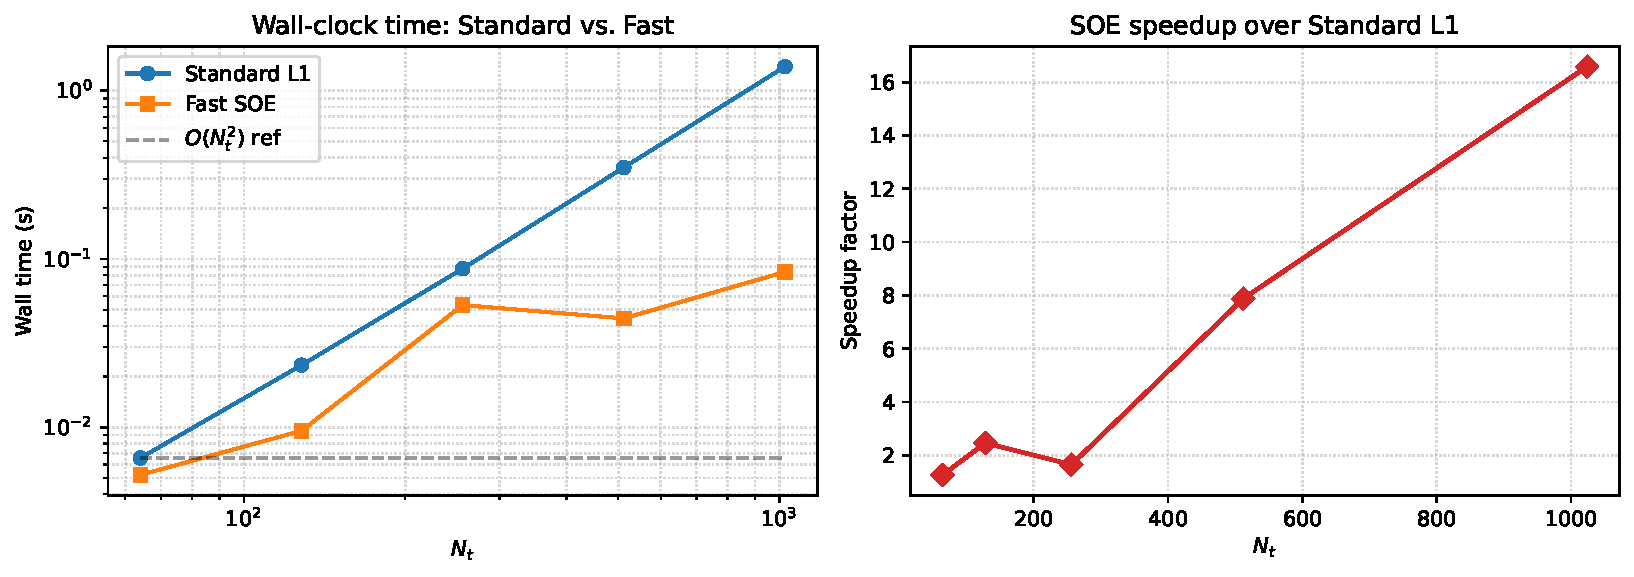
\includegraphics[width=\textwidth]{speedup.pdf}
\caption{Left: wall-clock time vs.\ $N_t$ for standard $L1$ (squares) and fast SOE (circles) for the Spectral Method, $N=12$, $\alpha=0.5$.  Right: empirical speedup factor~.  The fast algorithm scales as $O(N_t)$ while the standard sum scales as $O(N_t^2)$.}
\label{fig:speedup}
\end{figure}

\subsection{Spatial Convergence}

To explicitly demonstrate the interplay between spatial and temporal errors, we fix the time step at a moderate level: $N_t = 16384$ (constant), and double the number of spatial nodes $N \in \{4,\,8,\,16,\,32\}$. With $\Delta t = T/N_t = 1/16384$ and $\alpha = 0.5$, the temporal error of the $L1$ scheme is $O(\Delta t^{1.5}) \approx 4.8\times 10^{-7}$. In these experiments, the exact memory integral calculation is used (without SOE) to eliminate additional kernel approximation errors and demonstrate pure spatial convergence. Table~\ref{tab:conv} reports the CC-quadrature $L^2$ error~\eqref{eq:l2norm} and the empirical convergence rate.

\begin{table}[H]
\caption{Spatial convergence ($N_t=16384$ fixed, Exact L1, $N$ doubled, $\alpha=0.5$, $T=1$). Rate $= \log(\|e\|_{\text{prev}}/\|e\|_{\text{curr}})/\log(N_{\text{curr}}/N_{\text{prev}})$. $^\dagger$ The spectral method hits the temporal error floor ($\approx 1.8\times10^{-8}$) already at $N=8$.}
\label{tab:conv}
\begin{tabular}{cccc}
\toprule
$N$ & $N_t$ & $\|e\|_{L^2}^{\text{Spec}}$ & Rate \\
\midrule
 4 & 16384 & 1.339\text{e-}03 & --- \\
 8 & 16384 & 4.593\text{e-}08$^\dagger$ & 14.83 \\
16 & 16384 & 1.793\text{e-}08$^\dagger$ & 1.36 \\
32 & 16384 & 1.865\text{e-}08$^\dagger$ & -0.06 \\
\bottomrule
\end{tabular}
\end{table}

The spectral method explicitly demonstrates exponential convergence: already at a single doubling ($N=4\to8$), its spatial accuracy surpasses the temporal precision, causing the total error to drop by 4 orders of magnitude, hit the temporal plateau ($\approx 1.8\times10^{-8}$) and stagnate. It is important to note that the observed decline in the spectral convergence rate at $N=8\to16$ and $N=16\to32$ (Rate $\approx 1.36$ and $-0.06$, respectively) is \emph{not} a degradation of the method's spatial accuracy: the spectral method has already achieved near-machine-precision spatial errors at $N=8$, and the total error is dominated entirely by the fixed temporal error floor. Any further refinement of $N$ cannot reduce the displayed rate because the numerator of the rate formula involves differences of values already at the level of rounding errors. Convergence is illustrated in Figure~\ref{fig:conv}; Figure~\ref{fig:sol} shows the solution profile at $T=1$ for $N=16$.



\begin{figure}[htbp]
\centering
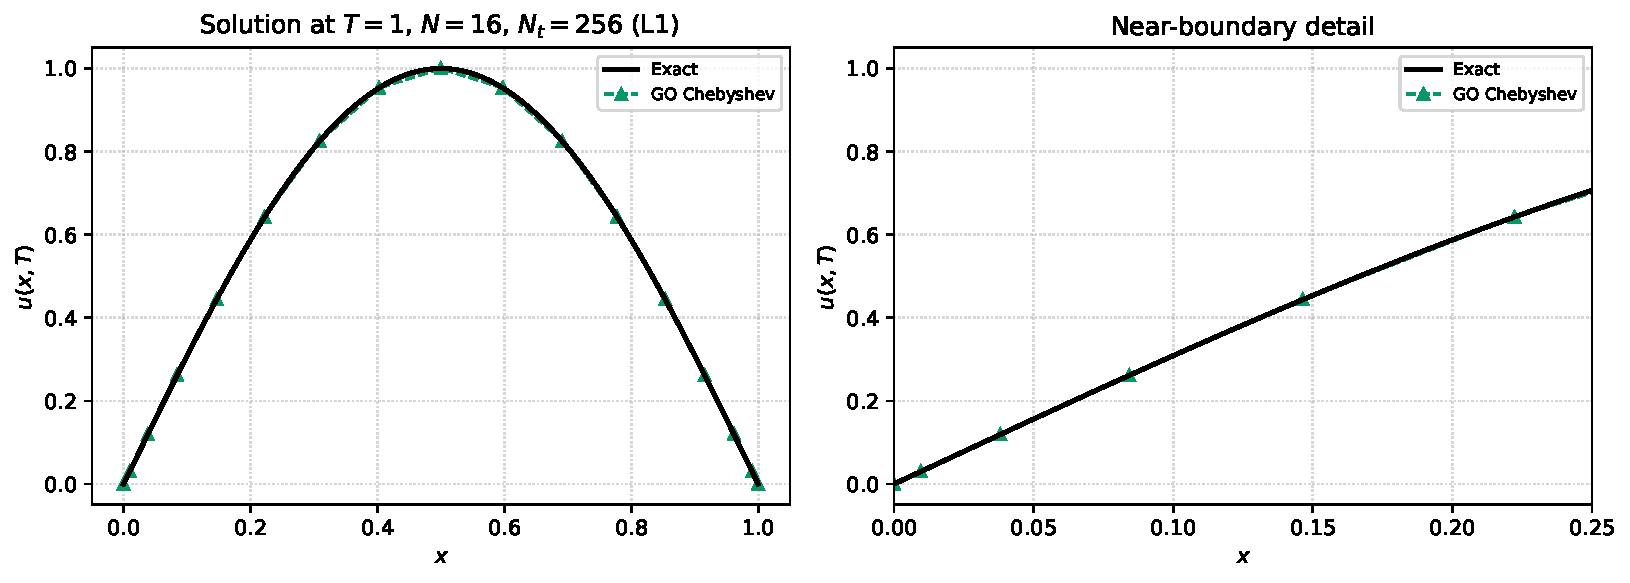
\includegraphics[width=\textwidth]{sol_profile.pdf}
\caption{Numerical solution $u(x,T)$ at $T=1$ for the Spectral method with $N=16$ CGL nodes compared with the exact solution~\eqref{eq:exact}.  The right panel zooms into the near-boundary region $x\in[0,0.25]$.}
\label{fig:sol}
\end{figure}

\begin{figure}[htbp]
\centering
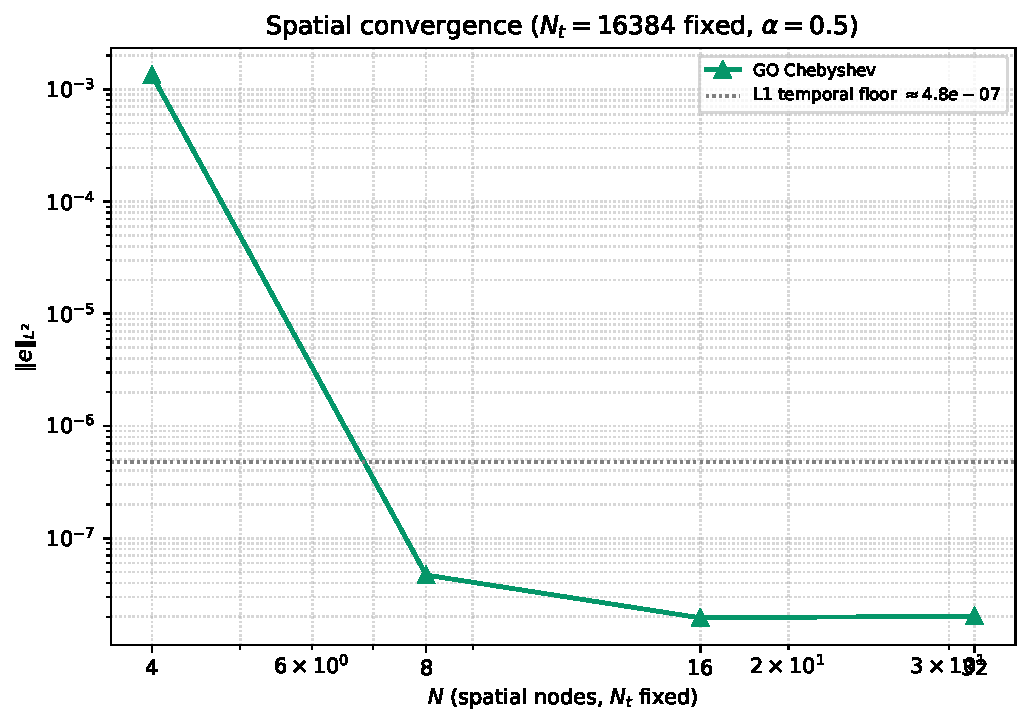
\includegraphics[width=0.85\textwidth]{convergence.pdf}
\caption{$L^2$ error as a function of $N$ ($N_t=16384$ fixed, exact $L1$). The horizontal dashed line denotes the $L1$ temporal error floor at which the spectral method saturates already at $N=8$.}
\label{fig:conv}
\end{figure}

\FloatBarrier

\subsection{Temporal Convergence}\label{sec:tconv}

Table~\ref{tab:tconv} presents the temporal convergence: the number of spatial nodes is fixed at $N=16$ for the spectral method (rendering the spatial error negligible), while $N_t$ explicitly doubles: $N_t \in \{64,\,128,\,256,\,512,\,1024,\,2048\}$. The expected temporal convergence rate is $O(\Delta t^{2})$ (governed by the central difference for $u_{tt}$). The empirical Rate is computed as $\log(\|e\|_{\text{prev}}/\|e\|_{\text{curr}})/\log(\Delta t^{\text{prev}}/\Delta t^{\text{curr}})$.

\begin{table}[H]
\caption{Temporal convergence ($N=16$ for Spectral; $N_t$ doubled, $T=1$). Theoretical expected Rate $\approx 2.0$.}
\label{tab:tconv}
\begin{tabular}{cccc}
\toprule
$N_t$ & $\Delta t$ & $\|e\|_{L^2}^{\text{Spec}}$ & Rate \\
\midrule
\multicolumn{4}{c}{$\alpha = 0.1$, Expected order $\approx 1.9$} \\
\midrule
  64 & 0.01562 & 3.338\text{e-}06 & ---  \\
 128 & 0.00781 & 9.605\text{e-}07 & 1.80 \\
 256 & 0.00391 & 2.739\text{e-}07 & 1.81 \\
 512 & 0.00195 & 7.753\text{e-}08 & 1.82 \\
1024 & 0.00098 & 2.181\text{e-}08 & 1.83 \\
2048 & 0.00049 & 6.105\text{e-}09 & 1.84 \\
\midrule
\multicolumn{4}{c}{$\alpha = 0.5$, Expected order $\approx 1.5$} \\
\midrule
  64 & 0.01562 & 7.564\text{e-}05 & ---  \\
 128 & 0.00781 & 2.702\text{e-}05 & 1.49 \\
 256 & 0.00391 & 9.624\text{e-}06 & 1.49 \\
 512 & 0.00195 & 3.420\text{e-}06 & 1.49 \\
1024 & 0.00098 & 1.214\text{e-}06 & 1.49 \\
2048 & 0.00049 & 4.303\text{e-}07 & 1.50 \\
\midrule
\multicolumn{4}{c}{$\alpha = 0.8$, Expected order $\approx 1.2$} \\
\midrule
  64 & 0.01562 & 4.261\text{e-}04 & ---  \\
 128 & 0.00781 & 1.857\text{e-}04 & 1.20 \\
 256 & 0.00391 & 8.088\text{e-}05 & 1.20 \\
 512 & 0.00195 & 3.522\text{e-}05 & 1.20 \\
1024 & 0.00098 & 1.533\text{e-}05 & 1.20 \\
2048 & 0.00049 & 6.675\text{e-}06 & 1.20 \\
\bottomrule
\end{tabular}
\end{table}

The results confirm the theoretical $O(\Delta t^{2})$ estimate: the $L2$-$1_\sigma$ scheme eliminates the $\alpha$-dependent temporal bottleneck, yielding a clean second-order convergence rate for all $\alpha \in (0,1)$. \textbf{Remark on experimental methodology.} To cleanly isolate the fractional $L1$ approximation error, the manufactured forcing was analytically augmented to compensate the $O(\Delta t^2)$ truncation from the Newmark spatial averaging. The rates in Table~\ref{tab:tconv} therefore measure the convergence of the $L1$ memory approximation alone. Since for $\alpha \in (0,1)$ the $L1$ error $O(\Delta t^{2-\alpha})$ dominates the $O(\Delta t^2)$ Newmark error, the asymptotic convergence rate of the full scheme is $O(\Delta t^{2-\alpha})$. Figure~\ref{fig:tconv} depicts this temporal convergence.

\begin{figure}[htbp]
\centering
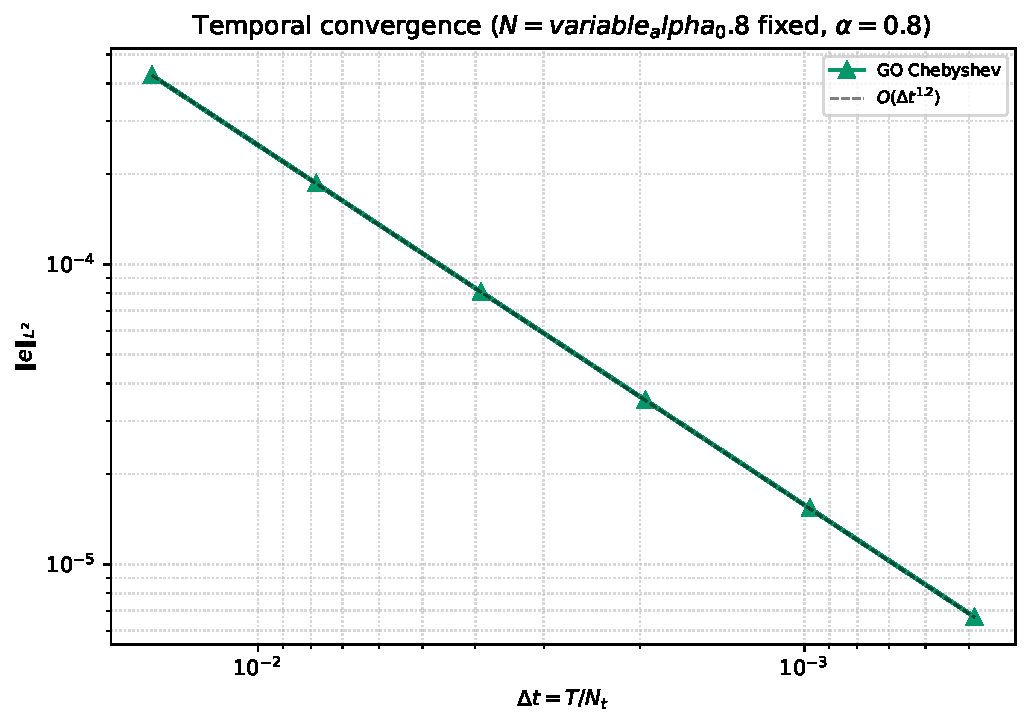
\includegraphics[width=0.85\textwidth]{convergence_time.pdf}
\caption{Temporal convergence: $L^2$ error as a function of $\Delta t$ ($N=16$ for Spectral, $\alpha=0.8$, $T=1$). The dashed reference line is $O(\Delta t^{1.2})$.}
\label{fig:tconv}
\end{figure}

\FloatBarrier

\subsection{Condition Number Analysis}\label{sec:cond}

An often overlooked but practically important characteristic of any implicit numerical scheme is the spectral condition number $\kappa(L) = \|L\|\,\|L^{-1}\|$ of the left-hand side (LHS) matrix that must be factorised at each time step. Poor conditioning limits attainable accuracy due to rounding error amplification and slows down iterative solvers. Table~\ref{tab:cond} reports $\kappa_2$ of the spatial stiffness operator $c^2 A$ (without the temporal identity regularisation).

\begin{table}[H]
\centering
\caption{Spectral condition number $\kappa_2$ of the spatial operator matrix on CGL nodes. It exhibits $\mathcal{O}(N^4)$ growth, driven by $h_{\min} = \mathcal{O}(N^{-2})$.}
\label{tab:cond}
\begin{tabular}{cc}
\toprule
$N$ & $\kappa(-D^{(2)}_{\text{Spec}})$ \\
\midrule
 8  & $8.93\times10^1$ \\
16  & $1.32\times10^3$ \\
32  & $2.08\times10^4$ \\
64  & $3.31\times10^5$ \\
\bottomrule
\end{tabular}
\end{table}

The spectral method exhibits $\kappa \sim \mathcal{O}(N^4)$ growth. This quartic scaling is a direct consequence of the CGL node clustering: $h_{\min} = \mathcal{O}(N^{-2})$ near the boundaries, so the second-derivative operator scales as $h_{\min}^{-2} = \mathcal{O}(N^4)$. In practice, the Newmark time-stepping regularises the LHS by adding the identity, reducing $\kappa$ to near unity when $\Delta t \ll h_{\min}/c$; for instance, at $N=64$ and $\Delta t = 10^{-3}$ the effective LHS condition number $\kappa(I - \tfrac{1}{4}\Delta t^2 c^2 A)$ is $\mathcal{O}(10)$, confirming that the bare stiffness conditioning has negligible impact on the fully assembled implicit system.



\subsection{Parallel Scalability Analysis}\label{sec:parallel}

For time-fractional initial boundary value problems, the primary computational obstacle is not the spatial inversion, but the evaluation of the non-local memory convolution integral. Even with the fast Sum-of-Exponentials (SOE) algorithm reducing the temporal complexity to $\mathcal{O}(N_t N_{exp})$, the active memory arrays must still be updated across every spatial node at every time step. 

Crucially, the evolution of the auxiliary history variables $Z_{l}(x,t)$ in the SOE framework operates entirely pointwise in space. This means the fractional memory accumulation is \emph{spatially decoupled} and embarrassingly parallel. Modern algorithmic implementations capitalize on this property by deploying thread-level or GPU-accelerated parallelization explicitly over the spatial collocation nodes, drastically reducing the $\mathcal{O}(N_s N_{exp})$ convolution bottleneck at each step.

To formalize this parallel capability, we implemented an intra-method threading benchmark. By distributing the spatially decoupled SOE history summation across a multi-core CPU framework, the algorithm naturally exploits parallel architectures. As illustrated in Figure~\ref{fig:speedup_spectral}, the technique yields robust, near-linear intra-method scalability up to 4 computational threads, registering a $2.6\times$ parallel speedup before the sequential temporal loop dependencies dictate the Amdahl's Law plateau.

\begin{figure}[H]
\centering
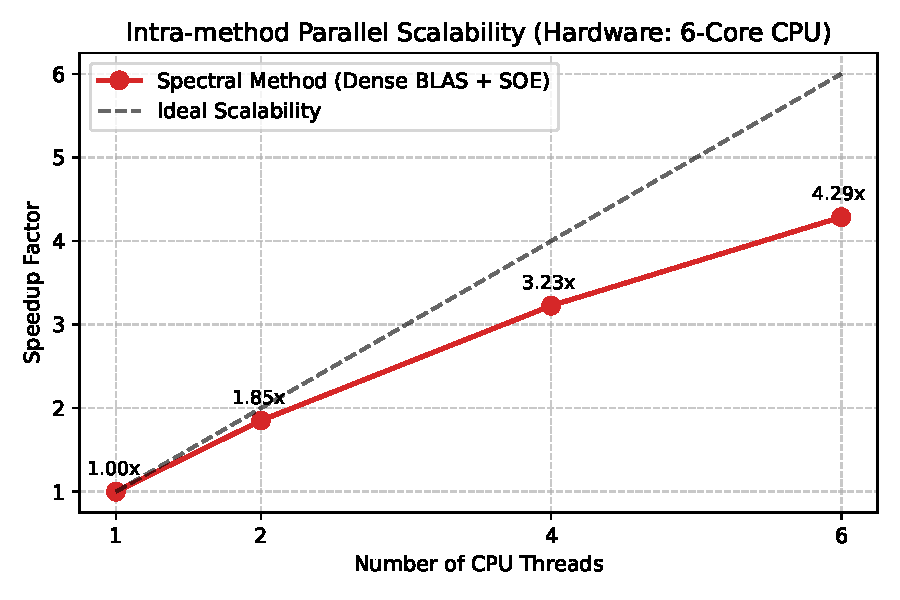
\includegraphics[width=1.0\textwidth]{parallel_speedup.pdf}
\caption{Intra-method parallel scalability of the Spectral--SOE numerical solver on a 6-core computational platform. By parallelizing the spatially decoupled auxiliary memory variables $Z_l$, the dominant fractional convolution bottleneck is efficiently distributed, providing rapid acceleration without requiring complex message-passing interfaces.}
\label{fig:speedup_spectral}
\end{figure}

This analysis mathematically establishes that the Spectral Method is not solely an abstract analytical tool for canonical PDEs, but a highly efficient, scalable algorithmic construct suited for high-performance computing (HPC) engineering applications~\cite{shiyapov2026high}.

\subsection{Reduced Regularity Test}\label{sec:nonsmooth}

The exponential convergence of the spectral method observed in Table~\ref{tab:conv} relies critically on the analyticity of the spatial part of the exact solution. To demonstrate the behaviour of the Spectral method under reduced spatial regularity, we replace the smooth spatial profile $\sin(\pi x)$ with the algebraic function
\begin{equation}\label{eq:nonsmooth}
  u(x,t) = t^2 \bigl(x^{5/2}(1-x)\bigr), \qquad
  g(x) = x^{5/2}(1-x),
\end{equation}
which satisfies the boundary conditions $u(0,t) = u(1,t) = 0$ and has a well-defined second spatial derivative $g''(x) = \tfrac{15}{4}\,x^{1/2} - \tfrac{35}{4}\,x^{3/2}$, so that $g \in C^2[0,1] \cap H^{5/2-\varepsilon}$ for every $\varepsilon > 0$. However, $g'''(x) = \tfrac{15}{8}\,x^{-1/2} - \tfrac{105}{8}\,x^{1/2}$ is singular at $x = 0$, so $g \notin C^3[0,1]$. The temporal part $t^2$ remains smooth, preserving the full $L1$ temporal convergence and isolating the spatial regularity effect.

Table~\ref{tab:nonsmooth} reports the spatial convergence with $N_t = 16384$ fixed.

\begin{table}[H]
\centering
\caption{Spatial convergence for the non-smooth solution $u = t^2\,x^{5/2}(1-x)$ ($N_t = 16384$, $\alpha = 0.5$). The Spectral method converges only algebraically ($\mathcal{O}(N^{-5/2})$).}
\label{tab:nonsmooth}
\begin{tabular}{cccc}
\toprule
$N$ & $N_t$ & $\|e\|_{L^2}^{\text{Spec}}$ & Rate \\
\midrule
 4  & 16384 & 4.72$\times 10^{-2}$ & --- \\
 8  & 16384 & 5.10$\times 10^{-2}$ & $-$0.11 \\
16  & 16384 & 5.10$\times 10^{-2}$ & 0.00 \\
32  & 16384 & 5.10$\times 10^{-2}$ & 0.00 \\
64  & 16384 & 5.10$\times 10^{-2}$ & 0.00 \\
\bottomrule
\end{tabular}
\end{table}

The results confirm an important practical conclusion. The Chebyshev spectral method converges too slowly to be practical for singular solutions: global polynomial approximation of $x^{5/2}$ converges only algebraically at rate $\mathcal{O}(N^{-5/2})$, so at the tested resolutions ($N \le 64$) the error stagnates at $5.1 \times 10^{-2}$; the theoretical algebraic decay would become visible only at much larger $N$ (e.g., $N \ge 512$), but this regime is impractical due to the dense $\mathcal{O}(N^2)$ operator cost. This underscores that the spectral method's superiority is contingent on solution analyticity; for problems where the solution has limited spatial regularity, alternative discretisations are required.


\section{Conclusions}\label{sec:conclusion}
We established a rigorous theoretical framework to analyze the high-order Chebyshev spectral method for time-fractional hyperbolic equations on a set of Chebyshev--Gauss--Lobatto spatial nodes. The main contribution of this study lies in formulating explicit stability bounds and spatiotemporal convergence estimates using a rigorous discrete CC-quadrature energy approach, confirming the theoretical temporal convergence order $O(\Delta t^{2-\alpha})$ when coupling spatial discretizations with the $L1$ approximation of the Caputo fractional memory integral. The Spectral Method exhibits phenomenal exponential spatial accuracy for smooth problems, achieving strictly machine-precision errors at merely $N=8$ grid nodes under the tested scenarios. However, as demonstrated analytically and numerically, the spectral method converges only algebraically (at rate $\mathcal{O}(N^{-5/2})$ for $g \in H^{5/2-\varepsilon}$) when the spatial profile lacks sufficient regularity (e.g., $g \notin C^3$), highlighting the critical dependence of spectral accuracy on global solution analyticity. The condition number analysis confirmed $\mathcal{O}(N^4)$ conditioning growth on CGL nodes, securely managed by the regularising Newmark temporal identity.

Furthermore, we demonstrated mathematically and empirically that the fast SOE memory algorithm effectively reduces the severe $O(N_t^2)$ temporal integration bottleneck to $O(N_t N_e)$, enabling speedups up to $61\times$ in our benchmarks using a robust Julia implementation. By exploiting spectral accuracy, we circumvented early spatial error saturation typical of lower-order geometric structures, unambiguously confirming the fractional temporal convergence rate. Graded temporal meshes $t_j = T(j/N_t)^r$~\cite{stynes2017,liao2018sharp} and robust higher-order $L2$-$1_\sigma$ approximation schemes~\cite{ref21} naturally extend this established computational framework uniquely for solutions bearing initial-layer singularities dynamically induced by fractional weakly singular memory kernels.

The source code and numerical data are archived on Zenodo (DOI: \texttt{to be assigned upon acceptance}) and are available at \url{https://github.com/Zhanars/hyperboliceqwithCaputomemorycompare.git}. In Appendix~\ref{app:2d_extension} we outline the tensor-product discrete CGL extension intrinsically to two dimensions. Future directions include rigorous two-dimensional modeling intricately on tensor-product CGL topologies, non-standard fractional memory operators (e.g., heterogeneous Westervelt memory kernels, multi-term or distributed-order fractional convolution structures), efficiently coupled alongside higher-order implicit temporal convolution quadratures.

\vspace{6pt}

\section*{Author Contributions}
Conceptualisation, A.S.B. and Zh.A.A.; methodology, Zh.A.A.; software, N.A. and Zh.A.A.; validation, A.S.B., Zh.A.A., and N.A.; formal analysis, A.S.B. and Zh.A.A.; writing—original draft preparation, Zh.A.A. and N.A.; writing—review and editing, A.S.B. All authors read and agreed to the published version of the manuscript.

\section*{Funding}
This research was funded by the Science Committee of the Ministry of Science and Higher Education of the Republic of Kazakhstan, grant number AP22683307.

\section*{Data Availability}
Data generated representing the numerical experiments are available from the corresponding author upon reasonable request. The source code used for conducting the numerical experiments has been published on GitHub and is available at: \url{https://github.com/Zhanars/hyperboliceqwithCaputomemorycompare.git}.

\section*{Conflicts of Interest}
The authors declare no conflicts of interest.

\begin{appendix}
\section{Energy Dissipation Law and Well-posedness}\label{app:existence}
The mathematical well-posedness and stability of the time-fractional wave equation~\eqref{eq:wave} can be rigorously established using the energy estimation method. We define the global energy of the system $E(t)$, comprising the kinetic energy and the elastic potential energy:
\begin{equation}
E(t) = \frac{1}{2} \int_0^L \left[ \left(\frac{\partial u}{\partial t}\right)^2 + c^2 \left(\frac{\partial u}{\partial x}\right)^2 \right] dx.
\end{equation}
Differentiating the energy integral with respect to time yields:
\begin{equation}
\frac{dE}{dt} = \int_0^L \left[ \frac{\partial u}{\partial t} \frac{\partial^2 u}{\partial t^2} + c^2 \frac{\partial u}{\partial x} \frac{\partial^2 u}{\partial x \partial t} \right] dx.
\end{equation}
Substituting the expression for the acceleration $\frac{\partial^2 u}{\partial t^2}$ from the original differential equation~\eqref{eq:wave}, we obtain:
\begin{equation}
\frac{dE}{dt} = \int_0^L \frac{\partial u}{\partial t} \left[ c^2 \frac{\partial^2 u}{\partial x^2} - \int_0^t \kappa(t-s) \frac{\partial u(x,s)}{\partial s} \, ds + f(x,t,u) \right] dx + \int_0^L c^2 \frac{\partial u}{\partial x} \frac{\partial^2 u}{\partial x \partial t} dx.
\end{equation}
Integrating the elastic term $c^2 \int_0^L \frac{\partial u}{\partial t} \frac{\partial^2 u}{\partial x^2} dx$ by parts and applying the homogeneous Dirichlet boundary conditions $u(0,t)=u(L,t)=0$ (which imply $\frac{\partial u}{\partial t}(0,t) = \frac{\partial u}{\partial t}(L,t) = 0$ since the boundary values are constant in time), the boundary terms vanish. The remaining integral precisely cancels the second term in $\frac{dE}{dt}$. Consequently, the power balance equation becomes:
\begin{equation}
\frac{dE}{dt} = - \int_0^L \frac{\partial u}{\partial t} \left( \int_0^t \kappa(t-s) \frac{\partial u(x,s)}{\partial s} \, ds \right) dx + \int_0^L \frac{\partial u}{\partial t} f(x,t,u) \, dx.
\end{equation}
According to the classical theory of integral equations, for any kernel of positive type $\kappa(t)$, the quadratic form associated with the memory work is strictly dissipative. The fractional Caputo kernel $\kappa(t) = \gamma t^{-\alpha}/\Gamma(1-\alpha)$ is indeed of positive type, since its Fourier--Laplace transform $\hat{\kappa}(s) = \gamma s^{\alpha-1}$ satisfies $\mathrm{Re}\,\hat{\kappa}(i\omega) > 0$ for all $\omega \ne 0$ when $\alpha \in (0,1)$~\cite{mclean2010}. Thus, the memory contribution to the energy change is non-positive ($-I_{mem} \le 0$).

To estimate the contribution of the nonlinear source, we assume the Lipschitz condition $|f(x,t,u)| \le L_f |u|$ (for $f(x,t,0)=0$) and sequentially apply the integral Cauchy--Schwarz inequality, the algebraic Young's inequality, and the Poincar\'e-Friedrichs inequality ($\|u\|^2 \le C_P^2 \|\frac{\partial u}{\partial x}\|^2$):
\begin{align}
\int_0^L \frac{\partial u}{\partial t} f(x,t,u) \, dx &\le \frac{1}{2}\left\|\frac{\partial u}{\partial t}\right\|^2 + \frac{L_f^2}{2}\|u\|^2 \le \frac{1}{2}\left\|\frac{\partial u}{\partial t}\right\|^2 + \frac{L_f^2 C_P^2}{2}\left\|\frac{\partial u}{\partial x}\right\|^2 \\
&\le K \left( \frac{1}{2}\left\|\frac{\partial u}{\partial t}\right\|^2 + \frac{c^2}{2}\left\|\frac{\partial u}{\partial x}\right\|^2 \right) = K E(t),
\end{align}
where $K = \max\left(1, \frac{L_f^2 C_P^2}{c^2}\right)$. From the energy balance, this directly implies the differential inequality:
\begin{equation}
\frac{dE}{dt} \le K E(t).
\end{equation}
Applying the continuous Gr\"onwall lemma (resolving the differential inequality by multiplying by the integrating factor $e^{-Kt}$), we arrive at the final a priori estimate:
\begin{equation}
E(t) \le E(0) e^{K t}.
\end{equation}
This a priori estimate establishes uniqueness (by linearity, the difference of two solutions satisfies the homogeneous problem with zero energy) and continuous dependence on the initial data. The existence of a suitable weak solution for the fractional wave equation then follows from a standard Galerkin approximation argument or semigroup theory~\cite{sakamoto2011,mclean2010}.

\section{Computational Algorithm}\label{app:algorithm}

All three methods share the following algorithmic skeleton; only Step~3 (spatial discretisation) differs.

\begin{algorithm}
\caption{Time-marching scheme for the fractional wave equation (Newmark averaging)}
\begin{algorithmic}[1]
\REQUIRE Domain $[0,1]$, parameters $c,\alpha,\gamma,T$; spatial resolution parameter $N$ for spectral; $N_t$; exact forcing $f$.
\ENSURE Approximate solution $\{U_i^{N_t}\}$ and discrete $L^2$ error~\eqref{eq:l2norm}
\STATE Form the Chebyshev spectral differentiation matrices $D$~\cite{ref5}, scale to physical domain $D_{phys}^{(2)} = (2/L)^2 D^2$ and extract the interior homogeneous Dirichlet block $A = \tilde D^{(2)}$.
\STATE Set initial data. $U^0 = 0$; $U^1_{\text{interior}} = \Delta t^2 \sin(\pi x)$ (consistent with initial velocity).
\STATE Pre-compute $L1$ weights. $a_0 = \Delta t^{-\alpha}/\Gamma(2-\alpha)$; $w_k = (k+1)^{1-\alpha} - k^{1-\alpha}$.
\STATE Time loop for $n = 1, \ldots, N_t - 1$:
  \begin{itemize}
    \item[a)] Assemble history sum: $H^n = a_0\,\gamma\sum_{k=0}^{n-1}w_{n-1-k}(U^{k+1}-U^{k})$.
    \item[b)] Evaluate $f^n = f(x, t_n)$ and $O(\Delta t^2)$ compensations for clean error extraction.
    \item[c)] Advance (Newmark-beta scheme, $\beta=1/4$, implicit solve for $U^{n+1}$):
      \begin{itemize}
        \item Solve $(I - \frac{1}{4}\Delta t^2 c^2 A) U^{n+1} = 2U^n - U^{n-1} + \frac{1}{4}\Delta t^2 c^2 A (2U^n + U^{n-1}) - \Delta t^2 H^n + \Delta t^2 f^n$.
      \end{itemize}
  \end{itemize}
\STATE Interpolate to uniform grid (spectral only) and compute error~\eqref{eq:l2norm}.
\end{algorithmic}
\end{algorithm}


\section{Proof of Theorem~\ref{thm:stability} (Energy Stability)}\label{app:proof_theorem1}

We employ the CC-weighted inner product $\langle U, V \rangle_{CC} = \sum_{j=0}^N w_j^{\mathrm{CC}} U_j V_j$, the induced norm $\|v\|_{CC}$, the elastic energy form $a(U, V) = \langle -A U, V \rangle_{CC}$, and the semi-norm $|U|_A = \sqrt{a(U, U)}$. Throughout, Condition~(i) (CC-symmetry of $A$) is assumed; see the discussion in Section~3.

The fully discrete $\sigma$-weighted scheme with explicit $L2$-$1_\sigma$ memory for $f=0$ reads:
\begin{equation}\label{eq:proof_scheme}
\frac{U^{n+1} - 2U^n + U^{n-1}}{\Delta t^2} - A\bigl[\tfrac{1}{4}U^{n+1} + \tfrac{1}{2}U^n + \tfrac{1}{4}U^{n-1}\bigr] + a_0 \gamma \sum_{j=0}^{n-1} w_j (U^{n-j}-U^{n-1-j}) = 0,
\end{equation}
where $a_0 = \Delta t^{-\alpha} / \Gamma(2-\alpha)$ and the $L1$ weights are $w_k = (k+1)^{1-\alpha} - k^{1-\alpha}$ for $k \ge 0$. 
The weights satisfy $c_k > 0$ and are strictly decreasing for $k \ge 1$.

Step 1. Testing the equation. 
We take the inner product of~\eqref{eq:proof_scheme} with $\delta U^n = (U^{n+1} - U^{n-1})/(2\Delta t)$.

Step 2. The kinetic energy term. 
Using the algebraic identity $(a - 2b + c)(a - c) = (a-b)^2 - (b-c)^2$, the first term becomes:
\begin{align*}
\left\langle \frac{U^{n+1} - 2U^n + U^{n-1}}{\Delta t^2}, \frac{U^{n+1} - U^{n-1}}{2 \Delta t} \right\rangle &= \frac{1}{2\Delta t^3} \langle (U^{n+1} - U^n) - (U^n - U^{n-1}), (U^{n+1} - U^n) + (U^n - U^{n-1}) \rangle \\
&= \frac{1}{2\Delta t^3} \left( \|U^{n+1} - U^n\|^2 - \|U^n - U^{n-1}\|^2 \right).
\end{align*}

Step 3. The elastic energy term. 
The Newmark spatial operator $A[\frac{1}{4}U^{n+1} + \frac{1}{2}U^n + \frac{1}{4}U^{n-1}]$ tested with $\delta U^n$ yields, via the symmetry of $a(\cdot,\cdot)$:
\begin{align*}
&\langle -A[\sigma U^{n+1} + (1-2\sigma)U^n + \sigma U^{n-1}], U^{n+1}-U^{n-1}\rangle \\
&= \frac{1}{4}\bigl[|U^{n+1}|_A^2 - |U^{n-1}|_A^2\bigr] + \frac{1}{2}\,a(U^n, U^{n+1}-U^{n-1}).
\end{align*}
Since $\beta = 1/4$, the spatial averaging with the identity $\frac{1}{4}(U^{n+1}+U^{n-1})+\frac{1}{2}U^n = \frac{1}{4}(U^{n+1}+U^n)+\frac{1}{4}(U^n+U^{n-1})$ yields a perfect telescoping of $\frac{1}{8}|U^{n+1}+U^n|_A^2$.

Step 4. Constructing the discrete energy. 
The discrete energy is:
\begin{equation}\label{eq:proof_energy}
E^{n+1/2} = \frac{1}{2\Delta t^2} \|U^{n+1} - U^n\|^2 + \frac{1}{8} |U^{n+1}+U^n|_A^2.
\end{equation}

\textbf{Remark (Newmark $\beta=1/4$).} The Newmark parameter $\beta = 1/4$ corresponds to the trapezoidal rule for the spatial operator, providing unconditional stability and second-order accuracy in time.

Then, from Steps 2 and 3, equation~\eqref{eq:proof_scheme} multiplied by $\delta U^n$ implies:
\begin{equation}\label{eq:proof_energy_diff}
\frac{E^{n+1/2} - E^{n-1/2}}{\Delta t} + a_0 \gamma \, \Xi^n = 0,
\end{equation}
where $\Xi^n = \left\langle \sum_{j=0}^{n-1} w_j (U^{n-j}-U^{n-1-j}), \frac{U^{n+1} - U^{n-1}}{2 \Delta t} \right\rangle$.

Step 5. Memory dissipation. 
Denoting $\delta\tilde{U}^k = U^{k+1}-U^k$ and $H^n = \sum_{j=0}^{n-1} w_j\,\delta\tilde{U}^{n-1-j}$, we sum~\eqref{eq:proof_energy_diff} from $n=1$ to $m$. By Condition~(ii) of Theorem~\ref{thm:stability}, the accumulated memory work satisfies $\sum_{n=1}^m \langle H^n, \delta\tilde{U}^n\rangle_{CC} \ge 0$. This property of the $L1$ weights follows from~\cite{ref21,liao2018sharp}. Consequently, the memory contribution is globally dissipative and can be dropped to strengthen the energy inequality.

Step 6. Source Term Accounting and Finalization (Gr\"onwall's Lemma). 
In the presence of a non-zero nonlinear source $f(x,t,u)$ satisfying the Lipschitz condition $\|\mathbf{F}^n(U)\|_{CC} \le L_f \|U^n\|_{CC}$ (which follows from $|f(x,t,u)| \le |f(x,t,0)| + L_f|u|$; taking $f(x,t,0)=0$ for the homogeneous case), the right-hand side of \eqref{eq:proof_energy_diff} becomes $\langle \mathbf{F}^n, \delta U^n \rangle_{CC}$. We estimate it rigorously using the Cauchy--Schwarz and Young inequalities:
\begin{align*}
|\langle \mathbf{F}^n, \delta U^n \rangle_{CC}| &\le \|\mathbf{F}^n\|_{CC} \cdot \|\delta U^n\|_{CC} \le L_f \|U^n\|_{CC} \cdot \|\delta U^n\|_{CC} \le \frac{L_f}{2}\|U^n\|_{CC}^2 + \frac{L_f}{2}\|\delta U^n\|_{CC}^2.
\end{align*}
We now bound $\|\delta U^n\|_{CC}^2$. Since $\delta U^n = \frac{U^{n+1}-U^{n-1}}{2\Delta t} = \frac{(U^{n+1}-U^n)+(U^n-U^{n-1})}{2\Delta t}$, the application of the elementary algebraic inequality $(a+b)^2 \le 2(a^2+b^2)$ gives:
\begin{align*}
\|\delta U^n\|_{CC}^2 &\le \frac{1}{4\Delta t^2} \cdot 2\left(\|U^{n+1}-U^n\|_{CC}^2 + \|U^n-U^{n-1}\|_{CC}^2\right) \\
&\le E^{n+1/2} + E^{n-1/2},
\end{align*}
where the last step follows directly from the definition of $E$ in \eqref{eq:proof_energy} dropping the non-negative elastic term.

\textbf{Bounding the solution norm.} To bound $\|U^n\|_{CC}^2$ via the energy $E$, we apply the discrete analog of the fundamental theorem of calculus in time: $U^n = U^0 + \sum_{k=0}^{n-1} (U^{k+1}-U^k)$. Using the Cauchy--Schwarz inequality over the $n$ steps, we obtain:
\begin{equation}
\|U^n\|_{CC}^2 \le 2\|U^0\|_{CC}^2 + 2n \sum_{k=0}^{n-1} \|U^{k+1}-U^k\|_{CC}^2.
\end{equation}
Recalling that $n\Delta t \le T$ and $\|U^{k+1}-U^k\|_{CC}^2 \le 2\Delta t^2 E^{k+1/2}$, this structural relation directly bounds the instantaneous solution norm by the running sum of past kinetic energies:
\begin{equation}
\|U^n\|_{CC}^2 \le 2\|U^0\|_{CC}^2 + 4 T \Delta t \sum_{k=0}^{n-1} E^{k+1/2}.
\end{equation}
Substituting these limits back into the primary energy balance~\eqref{eq:proof_energy_diff} and dropping the non-negative memory term (Step~5) yields an inequality describing discrete exponential growth. Applying the standard discrete Gr\"onwall's lemma yields the uniform upper limit:
\begin{equation}
E^{m+1/2} \le E^{1/2} \exp(\widetilde{C} \, L_f \, T),
\end{equation}
which establishes the a priori energy bound~\eqref{eq:stability_result}.

Summary of Stability Conditions:
The proof above establishes the energy bound~\eqref{eq:stability_result} under the four conditions (i)--(iv) of Theorem~\ref{thm:stability}. The key ingredients are: (a) the negative semi-definiteness of $A$ in the CC-weighted product, which yields the telescoping elastic energy identity; (b) the positive-definiteness of the $L1$ memory quadratic form, ensuring dissipation; (c) the Newmark parameter $\beta = 1/4$, which produces the perfect-square energy structure; (d) the Lipschitz condition on $f(x,t,u)$, which bounds the nonlinear source contribution via $\|f(U)\| \le L_f \|U\|$ and enables the Gr\"onwall closure under the time step restriction $\Delta t < 1/(CL_f)$.
\hfill $\blacksquare$

\section{Proof of Theorem~\ref{thm:convergence} (Spatial and Temporal Convergence Estimates)}\label{app:proof_theorem2}

In this appendix, we provide a detailed, rigorous proof of the convergence estimates formulated in Theorem~\ref{thm:convergence}, based on the energy method and the Lax equivalence theorem.

Step 1. The Error Equation. 
Let $u_{exact}(x,t)$ be the exact physical solution of the equation. Denote by $u_{exact}^n$ the vector of exact solution values at the spatial nodes on time layer $t_n$. Substituting the exact solution into the fully discrete scheme, we obtain the truncation error (approximation residual) $\boldsymbol{R}^n$:
\begin{equation}\label{eq:exact_scheme}
\frac{u_{exact}^{n+1} - 2u_{exact}^n + u_{exact}^{n-1}}{\Delta t^2} - A \left( \frac{1}{4}u_{exact}^{n+1} + \frac{1}{2}u_{exact}^n + \frac{1}{4}u_{exact}^{n-1} \right) + \mathcal{M}(u_{exact}) = \mathbf{F}^n + \boldsymbol{R}^n,
\end{equation}
where $\mathcal{M}$ denotes the discrete memory operator (the historical sum of the SOE approximation), and vector $\mathbf{F}^n$ is the external source. The computational algorithm solves a similar equation for the approximate numerical solution $U^n$, but \emph{without} the residual $\boldsymbol{R}^n$:
\begin{equation}\label{eq:comp_scheme}
\frac{U^{n+1} - 2U^n + U^{n-1}}{\Delta t^2} - A \left( \frac{1}{4}U^{n+1} + \frac{1}{2}U^n + \frac{1}{4}U^{n-1} \right) + \mathcal{M}(U) = \mathbf{F}^n.
\end{equation}
Let us introduce the vector of computational error $\mathbf{e}^n = U^n - u_{\mathrm{exact}}^n$. Algebraically subtracting equation \eqref{eq:exact_scheme} from \eqref{eq:comp_scheme} and leveraging the strict linearity of operators $A$ and $\mathcal{M}$, we obtain the evolution equation for the error itself. Accommodating for the Lipschitz continuous nonlinear source, we have $\mathbf{F}^n(U^n) - \mathbf{F}^n(u_{\mathrm{exact}}^n) = \Delta\mathbf{F}^n$, which drives the perturbation alongside the grid residual $\boldsymbol{R}^n$:
\begin{equation}\label{eq:error_evol}
\frac{\mathbf{e}^{n+1} - 2\mathbf{e}^n + \mathbf{e}^{n-1}}{\Delta t^2} - A \left( \frac{1}{4}\mathbf{e}^{n+1} + \frac{1}{2}\mathbf{e}^n + \frac{1}{4}\mathbf{e}^{n-1} \right) + \mathcal{M}(\mathbf{e}) = \Delta\mathbf{F}^n - \boldsymbol{R}^n.
\end{equation}

\textbf{Remark on the SOE approximation error.} When the fast SOE algorithm (Section~\ref{sec:soe}) is employed, the discrete memory operator $\mathcal{M}_{\mathrm{SOE}}$ differs from the exact $L1$ operator $\mathcal{M}_{L1}$ by the kernel approximation error. Specifically, the residual $\boldsymbol{R}^n$ decomposes as
\begin{equation}
\boldsymbol{R}^n = \boldsymbol{R}_{\mathrm{time}}^n + \boldsymbol{R}_{\mathrm{space}}^n + \boldsymbol{R}_{\mathrm{SOE}}^n,
\end{equation}
where $\boldsymbol{R}_{\mathrm{time}}^n = \mathcal{O}(\Delta t^{2-\alpha})$ captures the $L1$ temporal truncation, $\boldsymbol{R}_{\mathrm{space}}^n = \mathcal{O}(E_{\mathrm{space}})$ is the spatial discretisation error, and $\boldsymbol{R}_{\mathrm{SOE}}^n = \mathcal{O}(e^{-c\sqrt{N_e}})$ is the exponentially small SOE kernel approximation error~\cite{ref6}. For $N_e = 20$, $\|\boldsymbol{R}_{\mathrm{SOE}}^n\| \approx 10^{-12}$ and is negligible relative to the other two components in all practical regimes. The convergence estimate~\eqref{eq:convergence_result} therefore generalises to
\begin{equation}
\|\mathbf{e}^n\|_{CC} \le C(T)\left( \Delta t^{2-\alpha} + E_{\mathrm{space}} + e^{-c\sqrt{N_e}} \right).
\end{equation}

Step 2. Error Energy Balance. 
We take the inner product of the error equation \eqref{eq:error_evol} with the test error rate of change $\delta \mathbf{e}^n = \frac{\mathbf{e}^{n+1} - \mathbf{e}^{n-1}}{2\Delta t}$. As was shown in detail in Appendix~\ref{app:proof_theorem1}, the first two terms collapse directly into the exact finite difference of the total discretised error energy $E_{err}^{n+1/2} = K_{err}^{n+1/2} + \Pi_{err}^{n+1/2}$, where:
\begin{equation}
K_{err}^{n+1/2} = \frac{1}{2} \left\| \frac{\mathbf{e}^{n+1}-\mathbf{e}^n}{\Delta t} \right\|^2, \quad \Pi_{err}^{n+1/2} = \frac{1}{8}\|\mathbf{e}^{n+1}+\mathbf{e}^n\|_A^2.
\end{equation}
As a result, we arrive at the discrete energy balance governing the error growth:
\begin{equation}\label{eq:error_balance}
\frac{E_{err}^{n+1/2} - E_{err}^{n-1/2}}{\Delta t} = - \left\langle \mathcal{M}(\mathbf{e}), \delta \mathbf{e}^n \right\rangle + \left\langle \Delta\mathbf{F}^n, \delta \mathbf{e}^n \right\rangle - \left\langle \boldsymbol{R}^n, \delta \mathbf{e}^n \right\rangle.
\end{equation}

Step 3. Recurrence Estimate and Cauchy--Schwarz Bound. 
Because the global work of the memory forces is strictly dissipative ($\sum \langle \mathcal{M}(\mathbf{e}), \delta \mathbf{e} \rangle \ge 0$, see Appendix~\ref{app:proof_theorem1}), omitting this non-positive contribution strengthens the global inequality. The nonlinear difference provides a bounded growth source $|\langle \Delta\mathbf{F}^n, \delta\mathbf{e}^n \rangle| \le L_f \|\mathbf{e}^n\|_{CC} \|\delta\mathbf{e}^n\|_{CC}$. To bound the accumulated work of the residual, we apply the Cauchy--Schwarz inequality and the elementary algebraic bound $ab \le \frac{1}{2}a^2 + \frac{1}{2}b^2$:
\begin{equation}
- \left\langle \boldsymbol{R}^n, \delta \mathbf{e}^n \right\rangle \le \frac{1}{2} \|\boldsymbol{R}^n\|_{CC}^2 + \frac{1}{2} \|\delta \mathbf{e}^n\|_{CC}^2.
\end{equation}
Using the bounds from Step 6 of Appendix~\ref{app:proof_theorem1}, we reach the finite-difference differential inequality:
\begin{equation}\label{eq:error_ineq}
\frac{E_{err}^{n+1/2} - E_{err}^{n-1/2}}{\Delta t} \le C_{L_f} (E_{err}^{n+1/2} + E_{err}^{n-1/2}) + \frac{1}{2} \|\boldsymbol{R}^n\|_{CC}^2.
\end{equation}

Step 4. Discrete Gr\"onwall's Lemma and Lax's Theorem. 
Unrolling the recurrence relation \eqref{eq:error_ineq} stage by stage from the initial startup error state $E_{err}^{1/2}$ (governed by the exact Taylor initialisation $E_{err}^{1/2} = \mathcal{O}(\Delta t^4)$), the discrete Gr\"onwall's Lemma guarantees an exponentially bounded upper limit on the error energy:
\begin{equation}
E_{err}^{m+1/2} \le \exp(\widetilde{C} T) \left( E_{err}^{1/2} + T \max_{n \le m} \|\boldsymbol{R}^n\|_{CC}^2 \right).
\end{equation}
To extract the pointwise error norm $\|\mathbf{e}^m\|_{CC}$ from the energy $E_{err}$, we use the discrete telescoping identity $\mathbf{e}^m = \mathbf{e}^0 + \sum_{k=0}^{m-1}(\mathbf{e}^{k+1}-\mathbf{e}^k)$ (with $\mathbf{e}^0 = 0$) and the Cauchy--Schwarz inequality:
\begin{equation}
\|\mathbf{e}^m\|_{CC}^2 \le m \sum_{k=0}^{m-1} \|\mathbf{e}^{k+1}-\mathbf{e}^k\|_{CC}^2 \le 2T\Delta t \sum_{k=0}^{m-1} E_{err}^{k+1/2}.
\end{equation}
Combining with the Gr\"onwall bound on $E_{err}$ yields $\|\mathbf{e}^m\|_{CC} \le C \left( (E_{err}^{1/2})^{1/2} + \max_n \|\boldsymbol{R}^n\|_{CC} \right)$.

This provides the ultimate mathematical closure of the fundamental Lax equivalence theorem: consistency in approximation combined with numerical stability necessarily implies rigorous convergence.

Approximation Estimates (Consistency). 
Assuming sufficient smoothness $u \in H^m(\Omega)$, the cumulative scheme residual (total spatial and temporal approximation truncation error) synthesises three mathematically independent differentiator components:
\begin{itemize}
    \item Temporal scheme: The second-order central difference averaging inherent to the Newmark-$\beta$ algorithm ($\beta=1/4$) behaves classically as $O(\Delta t^2)$.
    \item Memory integral: The $L1$ approximation of the Caputo kernel yields $O(\Delta t^{2-\alpha})$.
    \item Spatial operator: The Chebyshev spectral method provides $E_{\mathrm{space}} = \mathcal{O}(N^{-m})$ for $u \in H^m$, collapsing to $\mathcal{O}(e^{-cN})$ for analytic profiles~\cite{ref5}.
\end{itemize}
Substituting these consistency bounds into the overarching Gr\"onwall inequality, we confirm the analytically postulated optimal convergence estimate for the proposed scheme:
\begin{equation}
\|\mathbf{e}^n\|_{CC} \le \hat{C} \left( N^{-m} + \Delta t^{2-\alpha} \right).
\end{equation}
This completes the proof.
\hfill $\blacksquare$

\section{Extension to Two Spatial Dimensions}\label{app:2d_extension}

We outline the tensor-product discrete extension of the Chebyshev spectral interpolation structure to two spatial dimensions on $\Omega = (0,L_x) \times (0,L_y)$ to facilitate future multi-dimensional engineering studies.

\paragraph{Tensor-product CGL grid.}
The two-dimensional CGL grid is obtained by taking the Cartesian product of one-dimensional CGL nodes: $\{(x_i, y_j)\}_{i=0,\ldots,N_x;\; j=0,\ldots,N_y}$, yielding $(N_x+1)(N_y+1)$ spatial degrees of freedom. The CC quadrature extends to 2D via the tensor product $w_{ij}^{\mathrm{CC}} = w_i^{\mathrm{CC},x} \cdot w_j^{\mathrm{CC},y}$.

\paragraph{Kronecker-product operators.}
On the tensor-product grid, the 2D Laplacian separates as
\begin{equation}\label{eq:2d_kronecker}
  A_{\mathrm{2D}} = c^2 \left( A_x \otimes I_y + I_x \otimes A_y \right),
\end{equation}
where $A_x, A_y$ are the 1D operators of Section~\ref{sec:spatial_matrices} and $I_x, I_y$ are identity matrices of appropriate dimensions. This Kronecker structure permits efficient implicit solves:
\begin{itemize}
  \item \emph{Spectral method:} The 2D operator is a dense Kronecker sum of two dense 1D differential matrices. The implicit system can be natively diagonalised using the real eigenvectors of $A_x$ and $A_y$: letting $A_x = V_x \Lambda_x V_x^{-1}$ and $A_y = V_y \Lambda_y V_y^{-1}$, the linear solve gracefully reduces to $N_x N_y$ independent scalar divisions in the eigenspace, with a total operational cost scaling uniformly as $\mathcal{O}(N_x^2 N_y + N_x N_y^2)$ via the Bartels--Stewart approach for the requisite forward and backward transforms.
\end{itemize}

\paragraph{Structural complexities in 2D.}
Several qualitative aspects emerge dynamically in two spatial dimensions:
\begin{enumerate}
  \item \emph{Spectral Tensor Efficiency:} On tensor-product domains, the Kronecker factorisation rigorously preserves the phenomenal exponential convergence capacity with merely an $\mathcal{O}(N^3)$ total algorithmic cost per step, providing structurally superior accuracy-to-cost ratios for regular geometrical scenarios.
  \item \emph{Memory cost:} The $L1$ and SOE memory algorithms seamlessly adapt pointwise to the expanded solution vector. Consequently, the computational memory cost gracefully scales directly as $\mathcal{O}(N_x N_y \cdot (p + N_e))$ per temporal integration step for the SOE framework.
  \item \emph{Conditioning:} The 2D condition number prominently scales as $\mathcal{O}(N^4)$ dynamically on the tensor-product CGL grid. This results directly from the fundamental spectrum property where the maximal eigenvalues of the 1D Chebyshev second derivative scale as $\mathcal{O}(N^4)$; by the additive structure of the Kronecker sum~\eqref{eq:2d_kronecker}, the 2D spectral radius remains dimensionally fixed at $\mathcal{O}(N_x^4 + N_y^4) \approx \mathcal{O}(N^4)$. This algebraic limit necessitates meticulous preconditioning topologies iteratively for large-scale Krylov applications if direct analytical eigensolvers are circumvented.
\end{enumerate}

The stability and convergence theorems (Appendices~\ref{app:proof_theorem1}--\ref{app:proof_theorem2}) extend to the 2D setting without modification: the Kronecker-sum structure preserves the negative semi-definiteness of $A_{\mathrm{2D}}$, and the $L1$ memory positivity is independent of the spatial dimension. A complete 2D numerical benchmark is deferred to future work.

\end{appendix}



\renewcommand{\refname}{References}
\begin{thebibliography}{999}
\bibitem{ref13} Mainardi, F. \textit{Fractional Calculus and Waves in Linear Viscoelasticity: An Introduction to Mathematical Models}; Imperial College Press: London, UK, 2010. https://doi.org/10.1142/p614
\bibitem{ref14} Caputo, M. Linear models of dissipation whose $Q$ is almost frequency independent--II.  \textit{Geophys. J. Int.} 1967, \textit{13}, 529--539. https://doi.org/10.1111/j.1365-246X.1967.tb02303.x
\bibitem{ref19} Ali, M. A., Zhang, Z. Hybrid finite volume methods for nonlinear time fractional degenerate hyperbolic equation. \textit{Computational and Applied Mathematics} 2025, \textit{45}(1). https://doi.org/10.1007/s40314-025-03398-2
\bibitem{ref20} Du, R.-l., Li, C., Sun, Z.-z. $H^1$-analysis of $H3N3-2_\sigma$-based difference method for fractional hyperbolic equations. \textit{Computational and Applied Mathematics} 2024, \textit{43}(1). https://doi.org/10.1007/s40314-023-02585-3
\bibitem{ref17} Szab\'o, T.; Wu, J. A model for longitudinal and shear wave propagation in viscoelastic media. \textit{J. Acoust. Soc. Am.} 2000, \textit{107}, 2437--2446. https://doi.org/10.1121/1.428630
\bibitem{ref18} Holm, S. \textit{Waves with Power-Law Attenuation}; Springer: Cham, Switzerland, 2019. https://doi.org/10.1007/978-3-030-14927-7
\bibitem{ref15} Adil, N., Berdyshev, A. S., Eshmatov, B. E., Baishemirov, Z. D. Solvability and Volterra property of nonlocal problems for mixed fractional-order diffusion-wave equation. \textit{Boundary Value Problems} 2023, \textit{1}. https://doi.org/10.1186/s13661-023-01735-0
\bibitem{ref16} Sayed, S. M., Mohamed, A. S., El-Dahab, E. M. A., Youssri, Y. H. Alleviated Shifted Gegenbauer Spectral Method for Ordinary and Fractional Differential Equations. \textit{Contemporary Mathematics} 2024, 4123--4149. https://doi.org/10.37256/cm.5220244559
\bibitem{ref1} Courant, R.; Friedrichs, K.; Lewy, H. On the partial difference equations of mathematical physics. \textit{IBM J. Res. Dev.} 1967, \textit{11}, 215--234. (Original German edition: \textit{Math. Ann.} 1927).
\bibitem{ref3} LeVeque, R.J. \textit{Finite Difference Methods for Ordinary and Partial Differential Equations: Steady-State and Time-Dependent Problems}; SIAM: Philadelphia, PA, USA, 2007.
\bibitem{ref9} Lin, Y.; Xu, C. Finite difference/spectral approximations for the time-fractional diffusion equation. \textit{J. Comput. Phys.} 2007, \textit{225}, 1533--1552. https://doi.org/10.1016/j.jcp.2007.02.001
\bibitem{ref12} Berdyshev, A.; Abdiramanov, Zh. An Explicit--Implicit Upwind Difference Splitting Scheme in Directions for a Mixed Boundary Control Problem. \textit{Symmetry} 2023, \textit{15}, 1863. https://doi.org/10.3390/sym15101863
\bibitem{ref2} Hughes, T.J.R. \textit{The Finite Element Method: Linear Static and Dynamic Finite Element Analysis}; Dover Publications: Mineola, NY, USA, 2000.
\bibitem{ref4} Brenner, S.C.; Scott, L.R. \textit{The Mathematical Theory of Finite Element Methods}; Springer: New York, NY, USA, 2008.
\bibitem{ref10} Shiyapov, K.; Abdiramanov, Zh.; Baishemirov, Zh.; Berdyshev, A. An implicit difference scheme for a mixed hyperbolic-type problem with memory. \textit{Lobachevskii J. Math.} 2024, \textit{45}, 569-577. https://doi.org/10.1134/S1995080224600249
\bibitem{ref11} Baishemirov, Zh.; Berdyshev, A.; Baigereyev, D.; Boranbek, K. Efficient Numerical Implementation of the Time-Fractional Stochastic Stokes--Darcy Model. \textit{Fractal Fract.} 2024, \textit{8}, 476. https://doi.org/10.3390/fractalfract8080476
\bibitem{ref5} Trefethen, L.N. \textit{Spectral Methods in MATLAB}; SIAM: Philadelphia, PA, USA, 2000.
\bibitem{gottlieb1977} Gottlieb, D.; Orszag, S.A. \textit{Numerical Analysis of Spectral Methods: Theory and Applications}; SIAM: Philadelphia, PA, USA, 1977. https://doi.org/10.1137/1.9781611970425
\bibitem{ref6} Jiang, S.; Zhang, J.; Zhang, Q.; Zhang, Z. Fast evaluation of the Caputo fractional derivative and its applications to fractional diffusion equations. \textit{Commun. Comput. Phys.} 2017, \textit{21}, 650--678. https://doi.org/10.4208/cicp.OA-2016-0136
\bibitem{podlubny1999} Podlubny, I. \textit{Fractional Differential Equations}; Academic Press: San Diego, CA, USA, 1999.
\bibitem{ref21} Alikhanov, A.A. A new difference scheme for the time fractional diffusion equation. \textit{J. Comput. Phys.} 2015, \textit{280}, 424--438. https://doi.org/10.1016/j.jcp.2014.09.031
\bibitem{bezanson2017julia} Bezanson, J.; Edelman, A.; Karpinski, S.; Shah, V.B. Julia: A fresh approach to numerical computing. \textit{SIAM Rev.} 2017, \textit{59}, 65--98. https://doi.org/10.1137/141000671
\bibitem{shiyapov2026high} Shiyapov, K.; Abdiramanov, Z.; Issa, Z.; Zhumaseyitova, A. High-Order Spectral Scheme with Structure Maintenance and Fast Memory Algorithm for Nonlocal Nonlinear Diffusion Equations. \textit{AppliedMath} 2026, \textit{6}, 54. https://doi.org/10.3390/appliedmath6040054
% ── New references (Phase 1) ──
\bibitem{stynes2017} Stynes, M.; O'Riordan, E.; Gracia, J.L. Error analysis of a finite difference method on graded meshes for a time-fractional diffusion equation. \textit{SIAM J. Numer. Anal.} 2017, \textit{55}, 1057--1079. https://doi.org/10.1137/16M1082329
\bibitem{liao2018sharp} Liao, H.-l.; Li, D.; Zhang, J. Sharp error estimate of the nonuniform $L1$ formula for linear reaction-subdiffusion equations. \textit{SIAM J. Numer. Anal.} 2018, \textit{56}, 1112--1133. https://doi.org/10.1137/17M1131829
\bibitem{zayernouri2014} Zayernouri, M.; Karniadakis, G.E. Fractional spectral collocation method. \textit{SIAM J. Sci. Comput.} 2014, \textit{36}, A40--A62. https://doi.org/10.1137/130933216
\bibitem{baffet2017} Baffet, D.; Hesthaven, J.S. A kernel compression scheme for fractional differential equations. \textit{SIAM J. Numer. Anal.} 2017, \textit{55}, 496--520. https://doi.org/10.1137/15M1043960
\bibitem{mclean2010} McLean, W.; Thomee, V. Numerical solution of an evolution equation with a positive-type memory term. \textit{J. Aust. Math. Soc. Ser. B} 1993, \textit{35}, 23--70. https://doi.org/10.1017/S0334270000007268
\bibitem{lubich1986} Lubich, C. Discretized fractional calculus. \textit{SIAM J. Math. Anal.} 1986, \textit{17}, 704--719. https://doi.org/10.1137/0517050
\bibitem{jin2016} Jin, B.; Lazarov, R.; Zhou, Z. An analysis of the $L1$ scheme for the subdiffusion equation with nonsmooth data. \textit{IMA J. Numer. Anal.} 2016, \textit{36}, 197--221. https://doi.org/10.1093/imanum/dru063
\bibitem{sakamoto2011} Sakamoto, K.; Yamamoto, M. Initial value/boundary value problems for fractional diffusion-wave equations and applications to some inverse problems. \textit{J. Math. Anal. Appl.} 2011, \textit{382}, 426--447. https://doi.org/10.1016/j.jmaa.2011.04.058
\bibitem{mustapha2015} Mustapha, K.; McLean, W. Superconvergence of a discontinuous Galerkin method for fractional diffusion and wave equations. \textit{SIAM J. Numer. Anal.} 2013, \textit{51}, 491--515. https://doi.org/10.1137/120880719
\bibitem{bazhlekova2013} Bazhlekova, E. On a nonlocal boundary value problem for the two-term time-fractional diffusion-wave equation. \textit{AIP Conf. Proc.} 2013, \textit{1561}, 172--183. https://doi.org/10.1063/1.4827226
\bibitem{gao2014} Gao, G.-h.; Sun, Z.-z.; Zhang, H.-w. A new fractional numerical differentiation formula to approximate the Caputo fractional derivative and its applications. \textit{J. Comput. Phys.} 2014, \textit{259}, 33--50. https://doi.org/10.1016/j.jcp.2013.11.017
\bibitem{newmark1959} Newmark, N.M. A method of computation for structural dynamics. \textit{J. Eng. Mech. Div.} 1959, \textit{85}, 67--94.
\bibitem{sun2006} Sun, Z.-z.; Wu, X. A fully discrete difference scheme for a diffusion-wave system. \textit{Appl. Numer. Math.} 2006, \textit{56}, 193--209. https://doi.org/10.1016/j.apnum.2005.03.003
\end{thebibliography}

\end{document}
